% cSpell:disable
% you should only have one "documentclass" line.  the following lines
% are samples that give various options.  the nofrontmatter option is
% nice because it suppresses the title and signature pages when you want
% to focus only on the main body of the thesis
%
% Friday April 10 2010 Ray Hylock <ray-hylock@uiowa.edu>
% documentclass options:
%   abstractpage            if you want to add an internal abstract (optional)
%   ackpage                 if you would like to add an acknowledgements page (optional)
%   algorithms              if you want a list of algorithms (optional)
%   appendix                if you have an appendix (optional)
%   copyrightpage           if you wish to copyright your thesis (optional)
%   dedicationpage          if you wish to make a dedication (optional)
%   epigraphpage            if you would like to add an epigraph to the beginning of your thesis (optional)
%   examples                if you want a list of examples (this uses the ntheorem package)
%   exampleslemmas          if you want a combined list of examples and lemmas (this uses the ntheorem package) (optional)
%   examplestheorems        if you want a combined list of examples and theorems (this uses the ntheorem package) (optional)
%   exampleslemmastheorems  if you want a combined list of examples, lemmas, and theorems (this uses the ntheorem package) (optional)
%   figures                 if you have any figures (this is required if you have even one figure)
%   lemmas                  if you want a list of lemmas (this uses the ntheorem package) (optional)
%   lemmastheorems          if you want a combined list of lemmas and theorems (this uses the ntheorem package) (optional)
%   nofrontmatter           suppresses the title and signiture pages for working on the body
%   tables                  if you have any tables (this is required if you have even one table)
%   theorems                if you want a list of theorems (this uses the ntheorem package) (optional)
%   phd                     if phd student; this will add the doctoral abstract (mandatory for PhD and DMA thesis candidates only)
%

% full options
%\documentclass[phd,abstractpage,copyrightpage,dedicationpage,epigraphpage,ackpage,figures,tables,lemmas,appendix]{uithesis}

% common options
%\documentclass[phd,dedicationpage,ackpage,figures,tables,appendix]{uithesis}

% example
\documentclass[phd,appendix,figures]{uithesis}

%=============================================================================
% User packages
%=============================================================================
\usepackage{bookmark}	% [recommended] for PDF bookmark generation
\usepackage{blindtext} 	% example text generation
\usepackage[ruled,chapter]{algorithm}  % display algorithms
\usepackage[super,comma,sort,numbers]{natbib}
\usepackage{amssymb}
% to place figures/subfigures
\usepackage{graphicx}
\usepackage{subfig}
% path to figures
\graphicspath{{notebooks/}{img/}{img/Aim1/}{img/Aim2/}{img/Aim3/}{img/CurrentStudy/}{img/GeneralDiscussion/}{img/GeneralMethods/}{img/Introduction/}}
\usepackage{forloop} % for loops display images
\usepackage{hyperref} % to insert hyperlinks
\usepackage{textcomp} % to write degree symbols
\usepackage{float} % image placement
% for smaller captions
\usepackage[labelfont=bf]{caption}
\captionsetup{font=footnotesize}
% https://tex.stackexchange.com/questions/370278/is-there-any-reason-to-use-inputenc
\usepackage[utf8]{inputenc} % for non-ascii characters
\newcommand{\comment}[1]{}
%=============================================================================
% prelude
%=============================================================================

\title{Task Related Correlations}
\author{James Kent}
\dept{Neuroscience}

% multipleSupervisors=true for two advisors
\setboolean{multipleSupervisors}{false}
\advisor{Assistant Professor Dr. Michelle Voss}
% for multiple advisors; change <value> to line up the names
%\setboolean{multipleSupervisors}{true}
%\advisor{Advisor 1\\\hspace{<value>mm}Advisor 2...}
%
% edit the names below to have your committee members names appear
% on the signature page.  memberOne should be your advisor.
%
\memberOne{Michelle Voss}
\memberTwo{Eliot Hazeltine}
\memberThree{Vincent Magnotta}
\memberFour{Jatin Vaidya}
\memberFive{Jan Wessel}
\submitdate{May 2020}
\copyrightyear{2020}

\Abstract{
\blindtext
}

%\dedication{Dedication here (optional)}

%\epigraph{Epigraph here (optional)}

%\acknowledgements{Acknowledgements here (optional)}

\begin{document}

\frontmatter
% cSpell:enable
%=============================================================================
\chapter{Introduction}
%=============================================================================

\begin{itemize}
	\item cognitive neuroscience draws line between brain/cognition
	\item tasks are necessary to understand how brain networks organize
	\item need to test methods that can measure brain organization
	\item two general methods are Beta Series Correlations and PsychoPhysiological Interactions
	\item Intro to BSC
	\begin{itemize}
		\item Jesse Rissman (2004): introduced LSA
		\item Jeanette Mumford (2012): introduced LSS
		\item introduce General Linear Model
		\item Benjamin Turner (2012)
		\item Abdulrahman (2016) compared LSA/LSS
	\end{itemize}
	\item Intro to PPI
	\begin{itemize}
		\item ppi's require three items in the model: psychological regressor, physiological regressor, and
		      interaction term of psychological/physiological term.
		\item 1997: Friston introduces ppi
		\item 2003: Geitman introduces deconvolution
		\item 2012: McLaren introduces gppi
		\item 2017: Di says to center psychological variable if performing deconvolution
		\item create psychological contrast of interest in the 2-condition experiment
		\item convolve the task design with the hrf, then multiply with bold signal
		\item for event related designs, deconvolve bold signal using basis functions,
			then multiply "neural" signal with task design (unconvolved), then convolve
			the neural ppi with the hrf
		\item create separate ppi's for each condition instead of creating a
		      new model for each contrast (gppi)
		\item denoise the seed region (include covariates in the basis functions)
		\item centering the psychological variable is necessary (or add deconvolve/reconvolved regressor)
	\end{itemize}
	\item previous work has compared LSA/LSS/PPI (Cisler 2014 and Xi 2020)
	\item comparisons missing LSS/LSA/PPI using mixed event/block design
	\item Intro to networks
	\begin{itemize}
		\item olaf sporns
		\item edge
		\item node
		\item simple network measures
	\end{itemize}
	\item I compared LSS/LSA first
	\item compare LSS/LSA relative to PPI
\end{itemize}
At the heart of any cognitive neuroscientist is the desire to relate the physical
processes of the brain to cognition.
The advent of functional Magnetic Resonance Imaging (fMRI) presented an amazing opportunity
to pursue the brain/cognition relationship like never before~\cite{ogawa1990}.
The serendipitous connection between blood rushing to areas of the brain where neurons
are working hardest provided the backdrop for discovering the large scale organization
of the brain and discovering which brain areas are recruited for specific tasks.
Another line of inquiry combines the previous questions to ask: How does the brain
organize to complete different tasks?
Instead of observing the brain's organization while there is no explicit task or observing
the whether a particular area is strongly recruited during a particular context,
answering the question how the brain organizes during a task represents our brain state
during the majority of our lives.
Whether it's writing an email, playing a card game, talking with colleagues; we are
often engaged in tasks throughout the day.
Thus, investigating how the brain organizes during a task grants understanding how
we operate in daily life.
What do I mean by organization?
For the context of this thesis, brain organization refers to which brain areas are communicating
with each other, which is measured by a statistical dependency between
regions like a Pearson's correlation.
The eagerness to understand brain organization during tasks has outpaced the investigations
of the methods to understand brain organization.
I compared different methods to measure brain organization during a task
and provide recommendations on which method to use.

Several methods have been introduced to measure brain organization during a task,
namely Beta Series Correlations (BSC) and Psychophysiological Interactions (PPI).
Their purpose is to measure task modulated differences in connectivity between brain areas.
In other words, they detect if the correlation between region A and B is different
in context 1 versus context 2.

Jesse Rissman :cite:`d-Rissman2004` was the first to publish on beta series
correlations, describing their usage in a working memory task.
In this task, participants saw a cue, a delay, and a probe, all occurring
within a short time period.
The cue was presented for one second, a delay occurred for seven seconds,
and a probe was presented for one second.
Given that the blood-oxygen-level-dependent (BOLD) response
takes approximately six seconds to reach its peak, and generally takes over
20 seconds to return to baseline, we can begin to see a problem.
The events within the events occur too close to each other to discern what
brain responses are related to encoding the cue, the delay, or the probe.
To discern how the activated brain regions form networks, Rissman
computed beta series correlations.
Instead of having a single regressor to describe all the cue events,
a single regressor for all the delay events, and a single regressor for all the
probe events (as is done in traditional task analysis),
there is an individual regressor for every event in the experiment.
For example, if your experiment has 40 events, each with a cue, delay, and
probe event, the model will have a total of 120 regressors, fitting a beta
(i.e., parameter) estimate for each event.
Once you calculate a beta estimate for each event of a given type
(e.g., cue), you will have a four-dimensional dataset where each volume
represents the beta estimates for a particular event.

Having one regressor per event in a single model is known as "least squares- all" (LSA).
This method, however, has limitations in the context of fast event-related
designs (e.g., designs where the events occur between 3-6
seconds apart on average).
Since each event has its own regressor, events that occur very close in time
are collinear (e.g., are very overlapping).

Jeanette Mumford :cite:`d-Mumford2012` derived a solution for
the high collinearity observed in least squares- all by using another
type of regression known as "least squares- separate" (LSS).
Instead of having one general linear model (GLM) with a regressor per event,
least squares- separate implements a GLM per event with only two regressors:
1) one for the event of interest, and 2) one for every other event in the
experiment.
This process reduces the collinearity of the regressors and creates a more valid
estimate for each trial, but also combines all other conditions
within the design matrix, which will reduce model fit.

Benjamin Turner :cite:`d-Turner2012a` improved upon the LSS method by retaining
the original conditions in the design matrix.
In this updated version, the individual trial's design matrix is almost the same
as the original design matrix, except that the trial is separated out into its
own regressor.

Benjamin Turner :cite:`d-Turner2012a` also adapted the LSS method by combining
it with finite impulse response (FIR) modeling, in which each of a set of
temporal delays following each trial is modeled as an impulse function in order
to characterize the shape of the BOLD response, as the
finite BOLD response- separate (FS) model.
The FS model showed promise as a method for decoding, as it does not make any
assumptions about the shape of the BOLD response.

NiBetaSeries can use the updated "least squares- separate" method,
the "finite BOLD response- separate" method, or the original
"least squares- all" method.

Psychophysiological Interactions (PPIs) are designed to 
identify brain areas that are differentially functionally connected
during specific contexts relative to others.
If this sounds like the same goal as BSC, you would be correct, although PPI
analyses take a different approach.
There are three necessary components to any PPI.
The first is the psychological variable of interest, such as when the participant
is responding to a congruent or incongruent event.
The second is the physiological variable, such as the BOLD signal from
the hippocampus.
The third variable is the PPI itself, which represents a multiplication
between the psychological variable and the physiological variable.
If our dependent variable is the BOLD signal in the medial frontal gyrus,
then we can answer the question if the hippocampus and medial frontal gyrus
are differentially functionally connected during congruent events relative
to incongruent events.

There are a couple of nuances worth addressing in the simplistic example I gave above.
First, there are likely multiple psychological conditions you would like to model.
In my above example, there were already two psychological conditions (congruent and incongruent)
to model.
Each pyschological condition is their own variable in the model, which also
means each condition has their own PPI.
In the example scenerio, there would be a total of 5 variables in the model,
two psychological variables for congruent and incongruent events,
one physiological variable for the hippocampal BOLD signal,
and two PPIs representing the multiplication between the hippocampal BOLD signal
and congruent and incongruent events.

The second nuance I would like to address is the multiplication between
the psychological and physiological variable.
The BOLD signal is the result of an underlying neural response convolved (i.e., smeared)
with a HRF.
\begin{equation}
	BOLD = HRF \circledast neural
\end{equation}
In order to multiply the BOLD signal with the psychological variable,
the psychological variable must go through the same convolution/smearing process.
\begin{equation}
	PSYCH_BOLD = HRF \circledast psych
\end{equation}
Brain-behavior interactions occur at the neural level, not at the
BOLD response level, as represented above.
Importantly, calculating the interaction at the BOLD level is not
equivalent to calculating the interaction the neural level.
\begin{equation}
	(HRF \circledast neural) \cdot (HRF \circledast psych) \neq HRF \circledast (neural \cdot psych)
\end{equation}
To get the neural signal we need to deconvolve the BOLD signal.
Deconvolution of the BOLD signal is not a well defined problem since
we do not know the exact neural process that gave rise to the BOLD signal.
Therefore we have to rely on regularized regression with an overcomplete
basis set.
Overcomplete meaning there are more columns (the basis set) than there
are rows (the BOLD signal).
Since the BOLD signal is noisy and assumed hemodynamic response function
may be significantly mis-shapen, some software packages simply do not attempt
deconvolution and swallow the error from multiplying the physiological and psychological
variables at the BOLD level.
Other software packages bite the bullet and attempt deconvolution.
In block designs where contexts are not intermixed the difference between
methods appears inconsequntial, but with rapid event-related designs,
deconvolution is essential to separate the influence of intermixed contexts.


Multiplying the physiological and psychological variables in BOLD space
is not mathematically equivalent to multiplication in neural space.

Evolution of Psychophysiological Interactions
\begin{itemize}
	\item 1997: Friston conceptualizes PPI
	\item 2003: Geitman introduces deconvolution
	\item 2012: McLaren introduces gppi
	\item 2017: Di says to center psychological variable if performing deconvolution
	\item create psychological contrast of interest in the 2-condition experiment
	\item convolve the task design with the hrf, then multiply with bold signal
	\item for event related designs, deconvolve bold signal using basis functions,
		  then multiply "neural" signal with task design (unconvolved), then convolve
		  the neural ppi with the hrf
	\item create separate ppi's for each condition instead of creating a new model for each contrast (gppi)
	\item denoise the seed region (include covariates in the basis functions)
	\item centering the psychological variable is necessary (or add deconvolve/reconvolved regressor)
	       
\end{itemize}


%=============================================================================
\chapter{Research Overview}
%=============================================================================

Advances in both fMRI analysis and theory of cognitive control have collided to produce ripe new areas to advance our understanding of cognitive control through fMRI ~\citep{Braver2012,Rissman2004,Mumford2012,Cisler2012}.
We can find evidence of cognitive control in our daily lives, from switching between an email and a conversation to making a quick decision behind the wheel. 
Specifically, cognitive control refers to the ability to use our context to inform our decisions. Cognitive control can be broken down into two modes, proactive and reactive ~\citep{Braver2012}. 
Proactive cognitive control encompasses the conflict preparation processes that occur for the entire duration of a task, and/or the conflict preparation between a cue and a stimulus.

In other words, the conflict processes that are not in direct response to a stimulus.
Reactive cognitive control, on the other hand, refers to the conflict adaptation that happens directly in response to a stimulus.
Two separable networks have been identified in proactive and reactive cognitive control, the cingulo-opercular (proactive) and fronto-parietal (reactive).
However, to this author's knowledge, there does not exist any research demonstrating the connectivity of these networks during a cognitive control task in fMRI.
Thus, the main thrust of this research is to establish these networks during a cognitive control task using two analytical methods theoretically sensitive to reactive or proactive cognitive control.

\begin{figure}[H]%
    \centering
    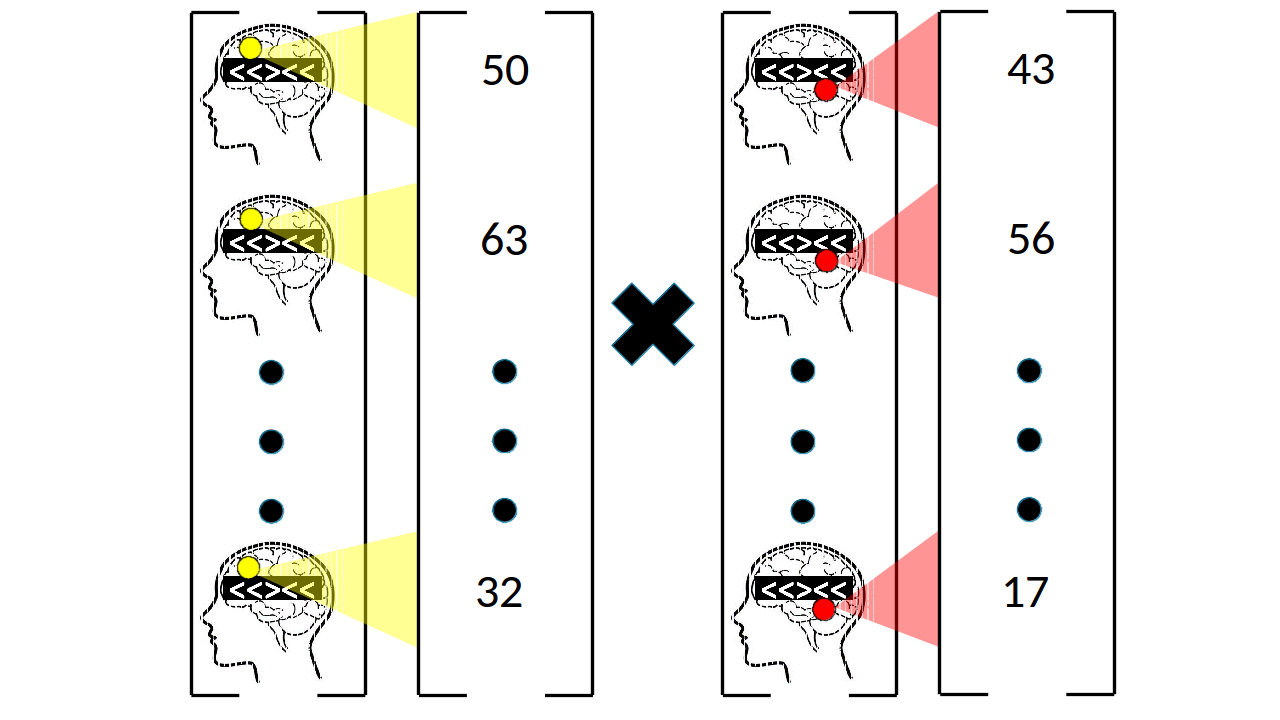
\includegraphics[scale=0.25]{betaseries_correlation_illustration}
    \caption{Setting up beta series Correlations. In the flanker task example above, betas (i.e. activation index) have been fit to every voxel per trial, and separated by condition (incongruent and congruent). This figure is only representing the incongruent trials, but both incongruent and congruent trial data can be collected.Regions of interest (ROIs) can be selected from these beta maps and all the voxels within the ROI are averaged. Once the betas are extracted from each ROI for each trial, the resulting lists of betas can be correlated with each other.}%
    \label{fig:betaseries_correlation_illustration}%    
\end{figure}

The first method is beta series correlations and is sensitive to the theoretical notion of reactive cognitive control (Figure ~\ref{fig:betaseries_correlation_illustration}). 
beta series correlations model the response after a congruent or incongruent stimulus capturing the "on-the-fly" conflict adaptations, otherwise known as reactive cognitive control.
Aim 1 will establish the use of this method due to its novel application to fast-event related designs of fMRI.

The second method is residual correlations; the time-course of the brain's activity after regressing out the stimulus onset information ~\citep{Fair2007,Cole2014,Bolt2017}. 
Residual correlations measure the theoretical notion of proactive cognitive control because proactive cognitive control represents the stable maintenance of goal-relevant task information throughout the performance of the task, which is what the time-series will represent.
Behavioral measures of proactive and reactive cognitive control exist, however outside of the AX-CPT it is difficult to analyze purely proactive and reactive behavioral components. 
Following the characterization of the purported reactive and proactive cognitive control networks, their relationship to existing behavioral measures will be established.
This research will contribute to the ongoing conversation of the neural basis of cognitive control, and provide a more direct metric of these networks during a  cognitive control task.

\section{Specific Aims}
\begin{figure}[H]%
	\centering
	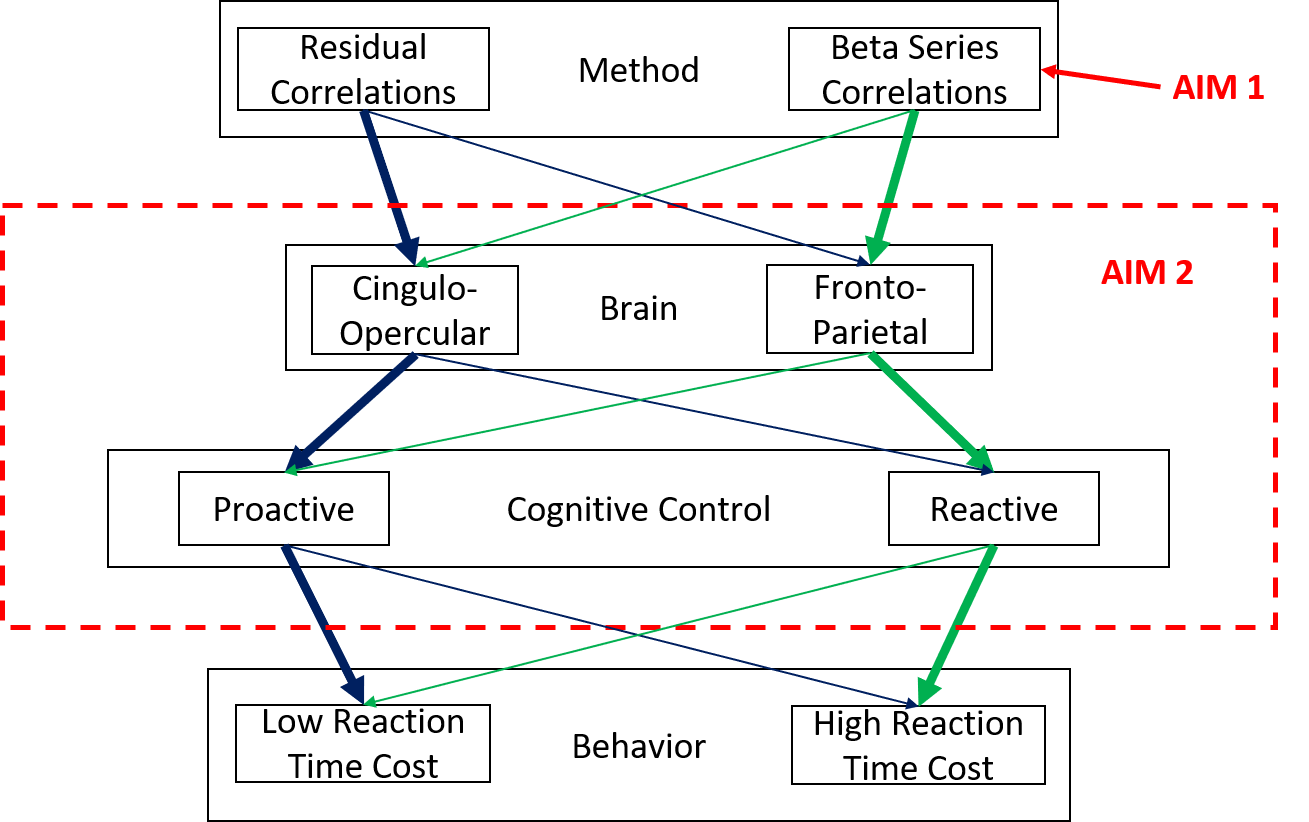
\includegraphics[width=1\linewidth]{overall_thesis_pic}
	\caption{Outline of my three aims. Aim 1 seeks to produce and validate software developed with nipype to perform beta series correlations.
	Aim 2 will profile beta series correlations and residual correlations on the same task datasets to derive differences and similarities between the methods and their relation to reaction time cost}
	\label{fig:all_aims}
\end{figure}

\textbf{Specific Aim 1}: Evaluate whether LSS or LSA is better
\newline
\newline
\textit{Rationale}: Should researchers reach to LSA for their analysis of condition specific differences
or should they use the more computationally intensive LSS?

\textit{Hypothesis}:
The beta series software will capture brain response variability across trials to produce correlations that are different from resting state correlations.
\newline
\newline
\textit{Method}:
Under the Nipype framework, I will use python to model data on a trial-by-trial basis ~\citep{Smith2004,Gorgolewski2017}. 
Using a traditional GLM with a double gamma basis function, modeling will be completed by performing a GLM for each trial individually, with all other trials of the same type combined into a single term to form a regressor of non-interest ~\citep{Mumford2012}.
Additionally, trials from other trial types will each get their own regressor.

Validation of the beta series software will be shown in three steps progressively from simulations to real data.
The first question I'm answering is \textbf{whether NiBetaSeries is able to capture BOLD response correlations.}
Starting from simulations, two voxels will be simulated with a specified correlation of BOLD responses that I control.
I will vary the correlation between the two voxels and inject different amounts of noise to ascertain how well nibetaseries recaptures the correlation I set between the two voxels.
From these simulations I will be able to approximate power for subsequent analyses.

\begin{figure}[H]%
	\centering
	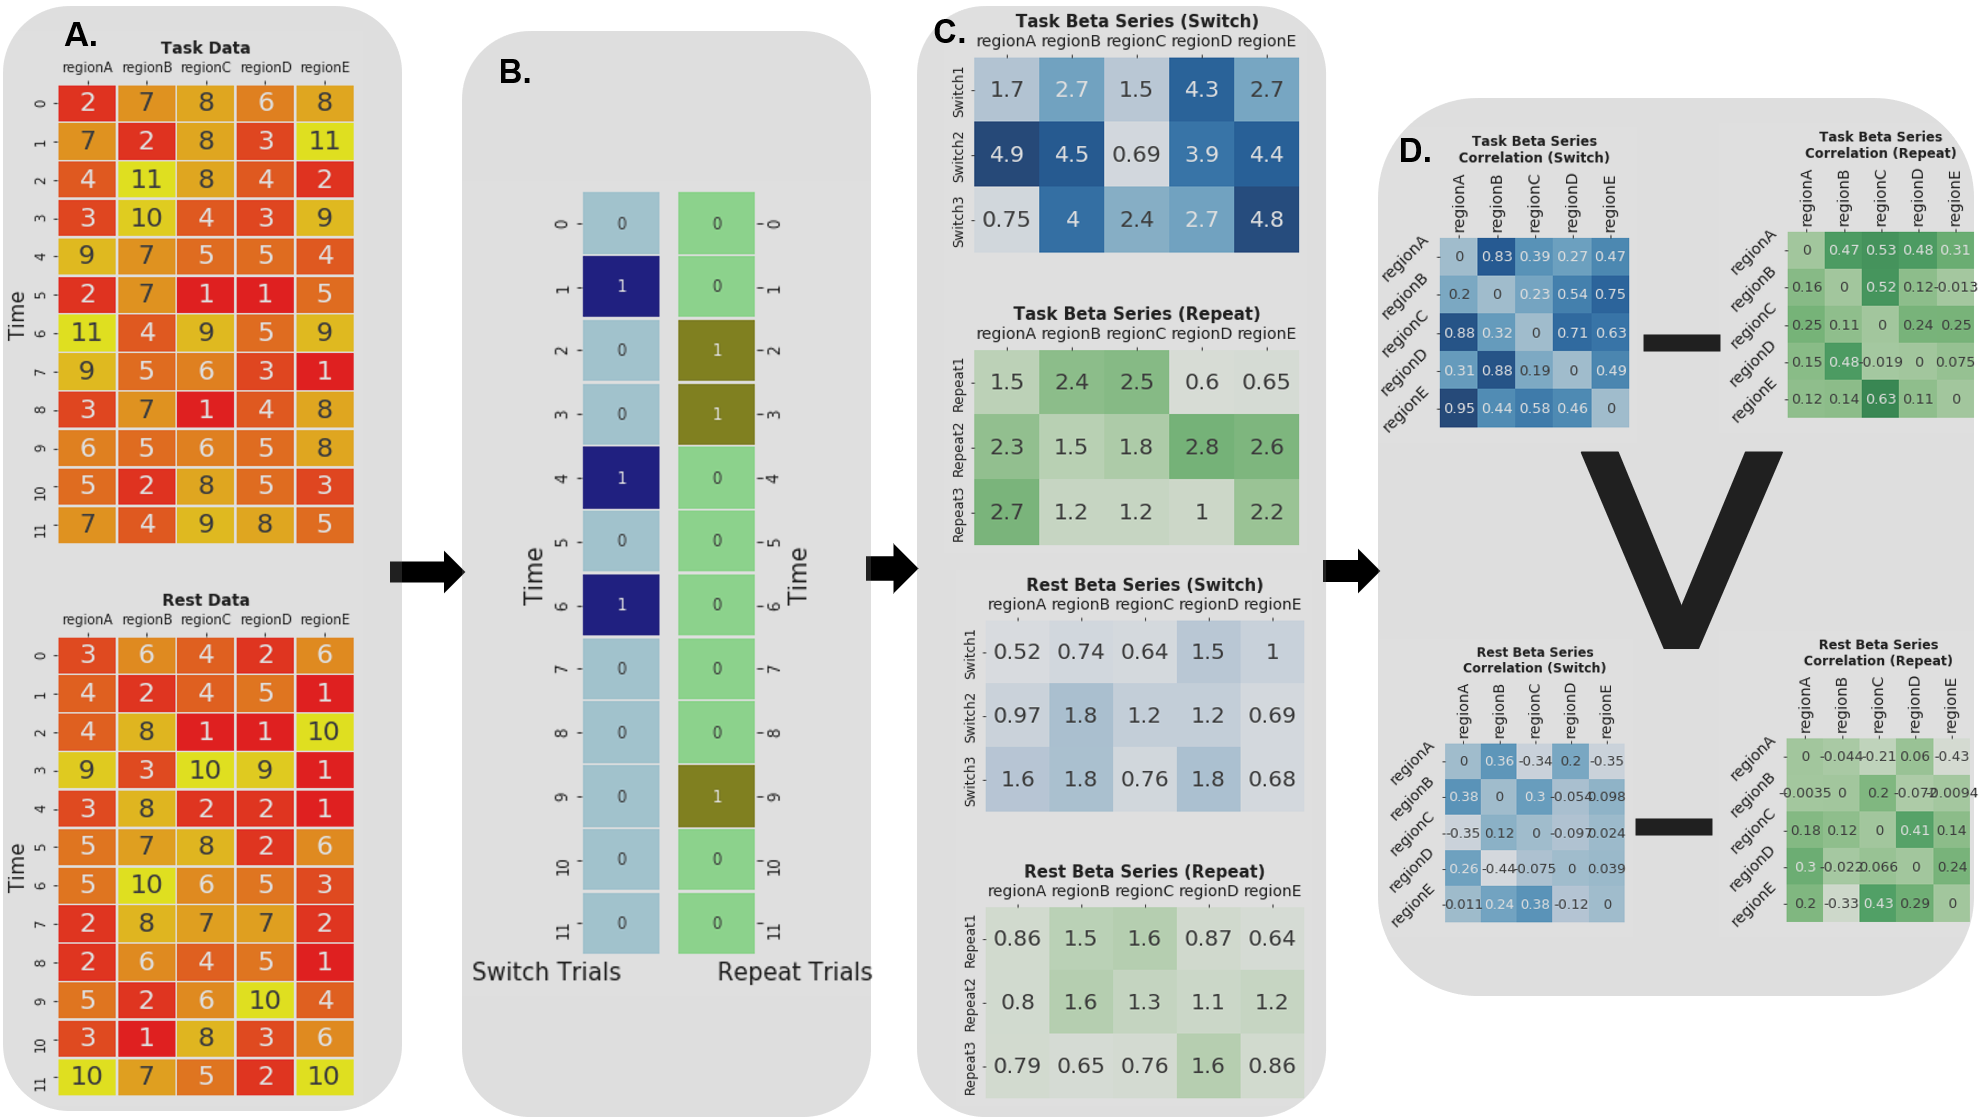
\includegraphics[width=1\linewidth]{validation_of_beta_series_pt_1}
	\caption{Applying Beta Series to both task and rest BOLD data.
	A) Flattened example task and resting state BOLD data are illustrated with 5 regions/voxels and 12 time points.
	Resting state data is being treated as if a task was performed.
	B) The two trial types in the task: switch and repeat. While the events did not actually occur during the resting state scan,
	I am treating the resting state data as though the events did occur.
	C) The expected betas series for the task and rest data.
	Note in the task data the switch trial type has higher betas on average relative to the repeat trial type.
	The trial types in the rest data should have similar betas since there was no actual task performed.
	D) The beta series are correlated between all regions for all trial types resulting in four 5x5 matrices.
	I expect the difference between the switch and repeat trial types in the task data to be greater than
	the difference between the switch and repeat trial types in the rest data.}
	\label{fig:validation_of_beta_series_pt_1}
\end{figure}

The second question I'm answering is \textbf{whether beta series correlations rely on the BOLD response to detect task-modulated differences}. 
The second validation will proceed by comparing task data with resting state data (Figure ~\ref{fig:validation_of_beta_series_pt_1}).
The resting state data will be analytically treated the same as the task data, testing the assertion nibetaseries uses the BOLD response to capture correlations between brain regions.
Brain regions and networks will be defined with the Schaefer 400 atlas ~\citep{schaefer2017}.
Beta series correlation matrices will be derived for repeat and switch trials separately for both task and rest resulting in four correlation matrices.
Beta series correlations will be averaged within the Schaefer control network, compressing the data to four observations per participant.
A linear mixed effects model will be run to test if the difference between switch and repeat can only be seen with the task beta series correlations.
The average correlation will be the dependent measure; data type (i.e., task or rest) and trial type (i.e., switch or repeat) will be the categorical predictors; and participant will have a random intercept.
I hypothesize there will be a significant interaction between data type and trial type where the difference between switch and repeat is greater for task beta series correlations relative to the rest beta series correlations.

\begin{figure}[H]%
	\centering
	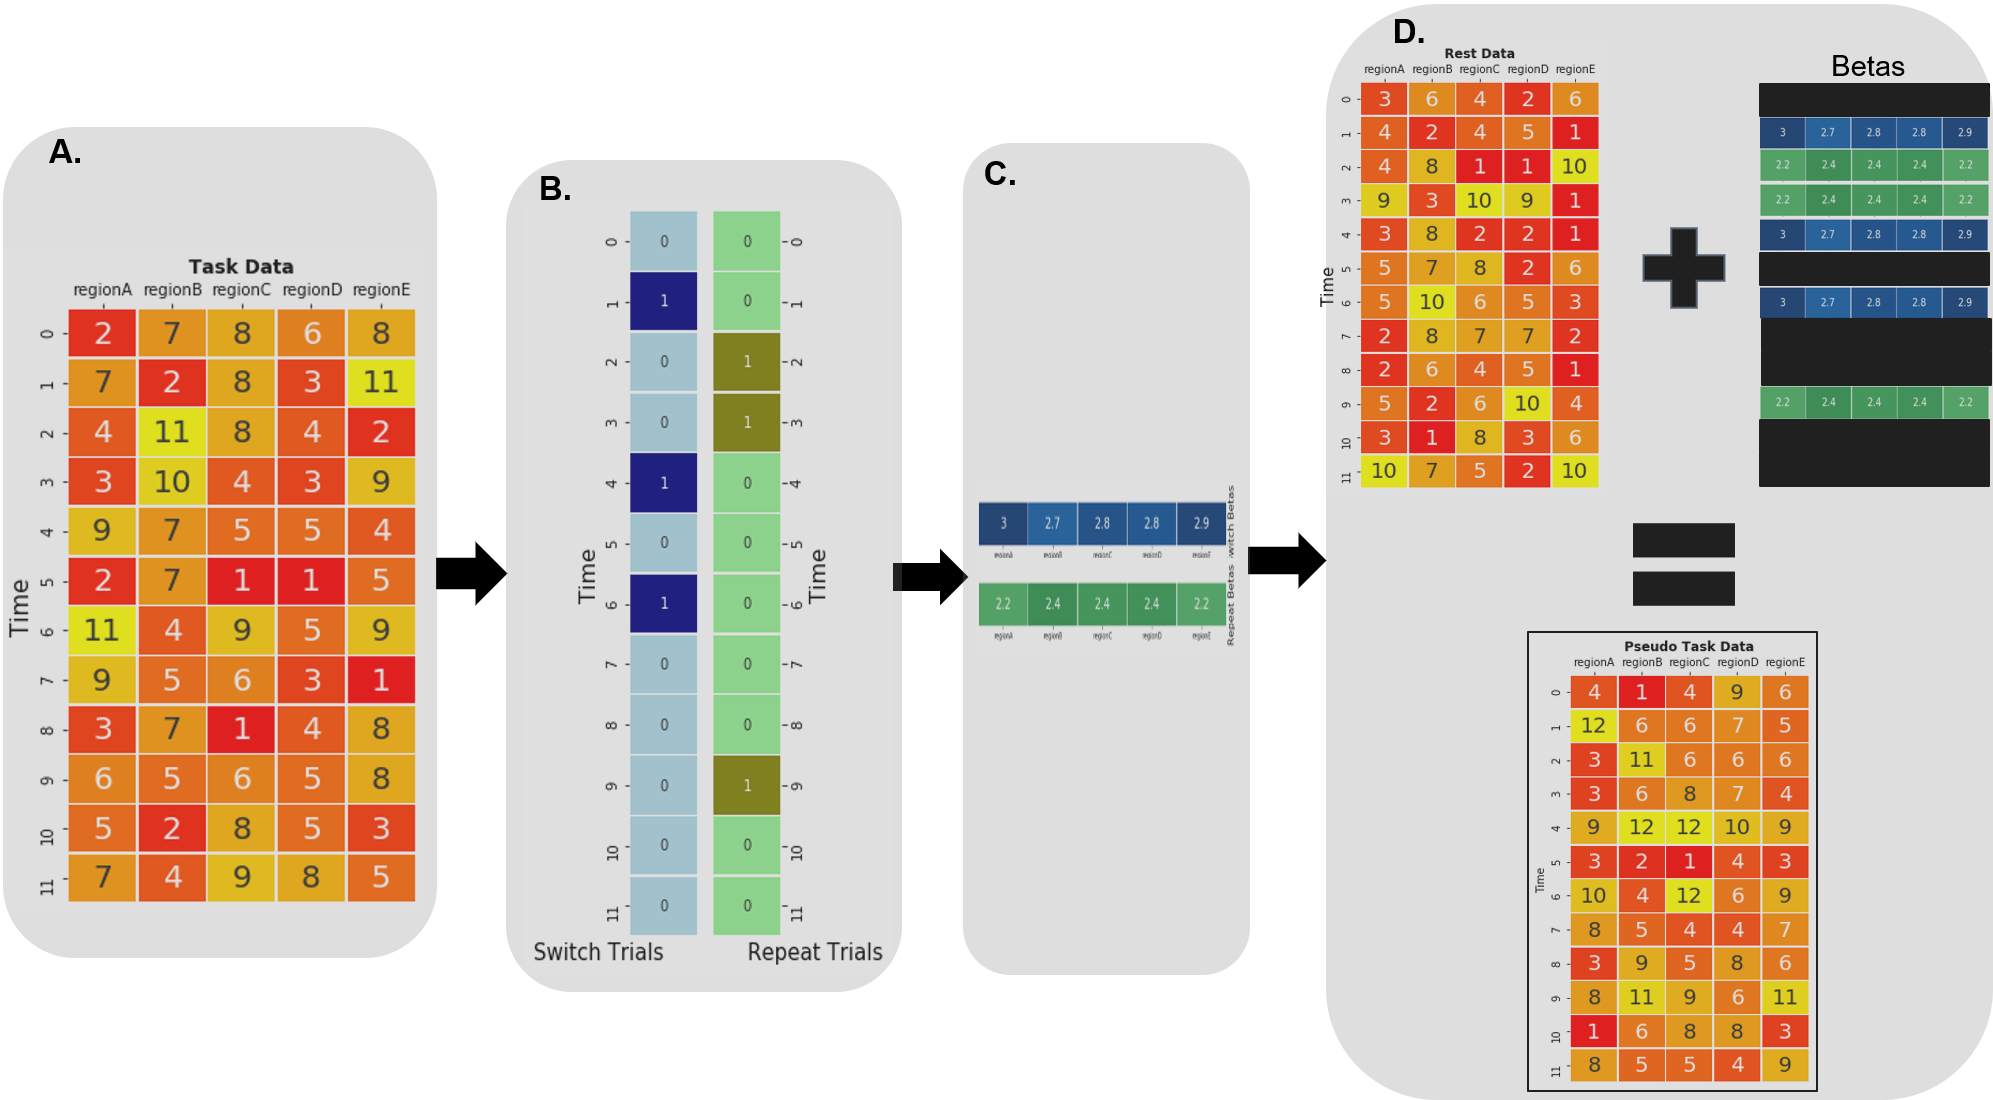
\includegraphics[width=1\linewidth]{validation_of_beta_series_pt_2}
	\caption{Creating Pseudo Task data from resting state data.
	A) Starting with the example flattened task BOLD data, B) calculate the average response of the task BOLD data
	to the two trial types (Switch and Repeat).
	C) Once the average responses (or betas) are calculated,
	D) I will take the resting state data and add the average responses back into the task BOLD data
	every time that trial type occurs.
	With the "pseudo-task" BOLD data, I can treat it as I would normal task BOLD data and calculate beta series
	correlations.
	}
	\label{fig:validation_of_beta_series_pt_2}
\end{figure}

The third question I'm answering is \textbf{if beta series correlations are driven by ongoing resting state fluctuations or by BOLD response variability dependent on task demands.}
BOLD response variability could merely be a reflection of ongoing resting state fluctuations and not a representation of brain reconfiguration driven by task demands (e.g., such as whether the trial type is switch or repeat).
If BOLD response variability is driven by resting state fluctuations, the difference in correlations between the switch and repeat trials would be attributable to the differences in response magnitude for each trial type.
In other words, the larger the BOLD response, the easier it is to detect the ongoing resting state correlations.
The third and final validation will be identical to the previous analysis, except the resting state data will have inserted task evoked responses creating “pseudo-task” data (Figure ~\ref{fig:validation_of_beta_series_pt_2}).
The resting state data will be convolved with a hemodynamic response that represents the average response for each unique trial type for a participant.
For every trial, the corresponding hemodynamic response for that trial type will be fit to every voxel.
If engaging in a task only adds BOLD responses to the ongoing resting state activity, the correlation matrices from the “pseudo-task” data and the task data should be close to each other.
However, if there is variance in the BOLD response that is independent of the ongoing resting state activity, the correlation matrices from the “pseudo-task” data and the task data should be different.
This test may provide evidence that beta series correlations capture unique variance not explained by resting state fluctuations, validating the utility of beta series correlations to answer novel questions about brain activity during a task.
\begin{figure}[H]%
	\centering
	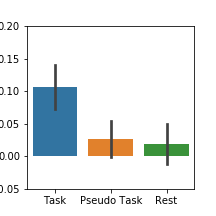
\includegraphics[width=1\linewidth]{aim_1_validation}
	\caption{Expected results from the real data validation.
	I expect the difference in beta series correlations between switch and repeat trial types should be the largest in the real task BOLD data and significantly greater than "pseudo-task" BOLD data and resting state BOLD data}
	\label{fig:aim_1_validation}
\end{figure}
The pattern of hypothesized trial-type differences for task, "pseudo-task" and rest is seen in Figure ~\ref{fig:aim_1_validation}.
\newline
\newline
\textit{Alternative Methods}: If the beta series approach introduces bias into the correlation measures (e.g., all regions are strongly correlated with each other), the method to derive betas will be re-evaluated.
If there is not a suitable method to reduce/remove the bias, psycho-physiological interactions (PPI) may be used instead to derive relative trial activation, although there is no a priori reason to believe PPI will be less susceptible to bias.
If averaging correlations within a network does not capture the data type by trial type interaction, multivariate methods may be used.
Specifically, a classifier could be trained on the correlation matrices to identify each of the categories (e.g., rest-switch, rest-repeat, task-switch, task-repeat)
leveraging the full correlation matrix.
Another option is to use graph theoretical measurements such as local or global efficiency to capture the state of overall network.
\newline
\newline
\textbf{Specific Aim 2}: Compare LSS/LSA to the standard method of PPI
\newline
\newline
\textit{Rationale}: The dual mechanisms of control theory posits these networks should be differentially sensitive to the type of correlation method applied ~\citep{Dosenbach2007,Braver2006}.
However, work by Michael Cole suggests there will not be large differences between residual correlations and beta series correlations ~\citep{Cole2019}.
Despite the suggestion by Michael Cole's work, the differences between residual correlations and beta series correlations have not been explicitly tested.
This gap presenting an excellent opportunity to conceptually frame task data into stimulus evoked components and persistent residual components.
\newline
\newline
\textit{Hypothesis}:
I hypothesize the cingulo-opercular network will be modulated by proactive cognitive control and will be detectable with residual time series, but not beta series.
My complementary hypothesis states the frontal-parietal network will be modulated by reactive cognitive control and will be detectable with beta series, but not residual time series. 
\newline
\newline
\textit{Methods}:
Data from the openneuro dataset \href{https://openneuro.org/datasets/ds001751/versions/1.0.0}{ds001751} will be used to measure both beta series and residual correlations during a Flanker task.
The task has two block types, mostly incongruent (80 percent incongruent) and mostly congruent (20 percent incongruent).
The mostly incongruent block incites proactive cognitive control because the participant is likely to have to resolve a stimulus conflict for each trial.
On the other hand, the mostly congruent block encourages reactive control because the participant is not likely to see a conflicting stimulus.
All participants went through both congruent and incongruent blocks constituting a fully within subjects design.
The behavioral results indicate a successful manipulation of the congruency effect ~\citep{Aben2019}.
The participants had a much smaller congruency effect (measured with reaction time series) during the mostly incongruent block relative to the mostly congruent block.
For each participant, I will be able to measure both beta series correlations and residual correlations during mostly incongruent blocks and mostly congruent blocks. 
Using the Dosenbach ROIs, I will create correlation matrices for both beta series and residual time series ~\citep{Dosenbach2010}.
I will test the robustness of the results using the Schaefer atlas as an alternative atlas ~\citep{schaefer2017}.

\begin{figure}[H]%
	\centering
	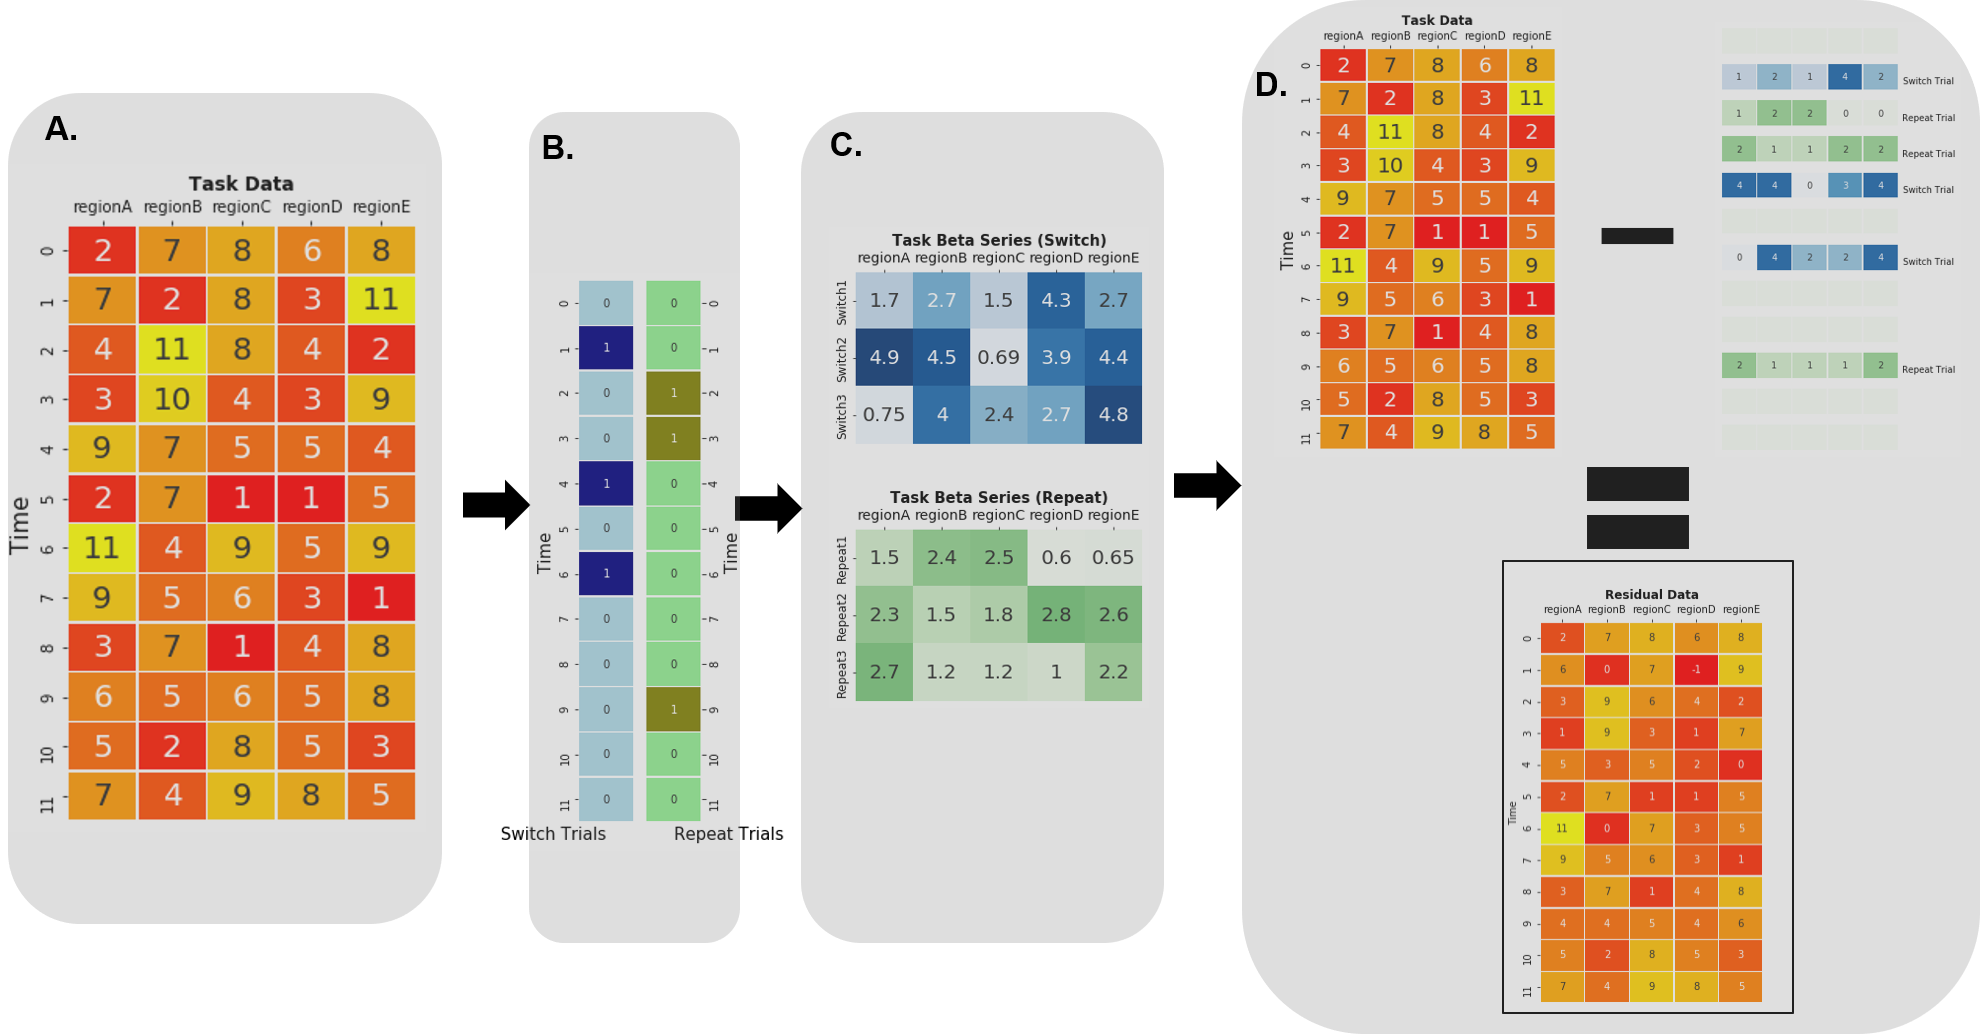
\includegraphics[width=1\linewidth]{residual_correlations}
	\caption{Calculating Residual Correlations.
	A) Flattened and simplified task BOLD data with 12 time points and 5 regions/voxels.
	B) Each trial onset will get its own regressor in a GLM to
	C) calculate an individual beta per trial, resulting in a beta series.
	D) The beta series will be subtracted from the original task BOLD data, removing potential
	trial modulated BOLD response variance, only leaving the variance attributed to task context (e.g., whether the block was congruent or incongruent).}
	\label{fig:residual_correlations}
\end{figure}

To calculate residual correlations four steps will be completed ~\ref{fig:residual_correlations}.
First, the stimulus responses will be modeled and removed from the data.
To remove the stimulus responses, stimulus onsets from the task will be represented as impulses and convolved with a double gamma as the basis function for the GLM. 
Each stimulus event will entered into the GLM as its own regressor.
This ensures the trial-to-trial variance will be removed from the task data, and not just the mean response of a stimulus. 
The residual data from the GLM will represent BOLD responses not captured by direct responses to stimuli. 
Second, the data will be split into the mostly congruent block and mostly incongruent blocks.
The splitting allows me to analyze the state dependent correlations during the mostly congruent and mostly incongruent blocks separately.
Third, the data will be z-transformed to normalize the distributions and Pearson's R correlations will be extracted from ROIs that participate in the fronto-parietal network and the cingulo-opercular network.
Fourth, ROIs that belong to the same network will be correlated with each other and averaged giving an average within network correlation.

Beta series will be calculated as described in aim 1.
The correlations will be performed similarly to the residual correlations, except instead of residuals, the beta maps will be normalized and within network correlations will be calculated for the incongruent trial type within the mostly incongruent and mostly congruent blocks.
Average within network correlations for the cingulo-opercular and fronto-parietal networks across participants for both beta series and residual correlations in the mostly incongruent block and mostly congruent block serve as the primary outcome measure.
I will look at change in within network correlations as a function of the network (fronto-parietal and cingulo-opercular) by block (mostly incongruent and mostly congruent) by method (residual and beta series correlations) using mixed effects modeling with a random intercept for participant.
I predict a significant network by block by method interaction ~\ref{fig:aim_2_validation}.
\begin{figure}[H]%
	\centering
	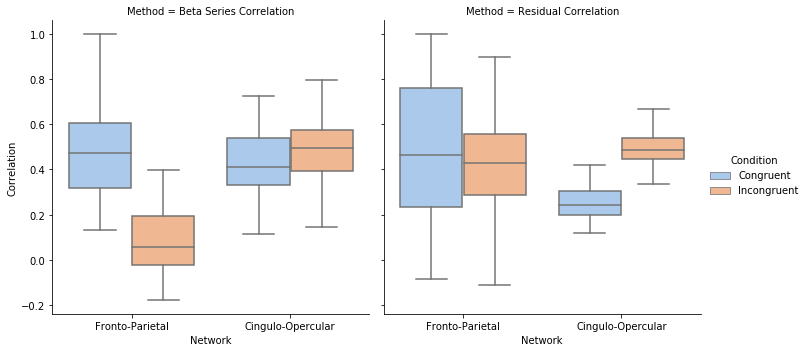
\includegraphics[width=1\linewidth]{aim_2_validation}
	\caption{Hypothesized relationship between network (fronto-parietal and cingulo-opercular), method (beta series and residual), and block (mostly congruent and mostly incongruent).
	I hypothesize the fronto-parietal network beta series correlation should be lower during the incongruent block relative to the congruent block.
	There is not a strong prediction on how the cingulo opercular network will behave with beta series correlations.
	I also hypothesize the cingulo-opercular network residual correlation should be higher during the incongruent block relative to the congruent block.
	There is not a strong prediction on how the fronto-parietal network will behave with residual correlations.}
	\label{fig:aim_2_validation}
\end{figure}
From this interaction I expect the within network residual correlations from the cingulo-opercular network to increase during the mostly incongruent block relative to the mostly congruent block.
This prediction supports the proactive role of the cingulo-opercular network which is proposed to be online during the entirety of the mostly incongruent block.
I also expect the within network beta series correlations from the fronto-parietal network to increase during the mostly congruent block relative to the mostly incongruent block.
This prediction supports the reactive role of the fronto-parietal network which is only called upon during the incongruent trials within the mostly incongruent block.
\newline
\newline
\textit{Alternative Methods}:
Beta series correlations give correlations for each trial type (incongruent and congruent), but in the proposed methods I only anticipate the incongruent trials to have explanatory power.
However, it could be the relationship between congruent and incongruent trial types changes between the blocks suggesting subtracting the congruent correlation matrix from the incongruent correlation matrix would be more sensitive to the difference between blocks.
The mixed effects regression may also contain quality metrics of the data including average framewise displacement and global correlation to rule out noise driving the observed effect. 
If within network correlations from mixed effects regression do not adequately model the differences, I can use graph theoretical measures such as participation coefficient and efficiency.
\newline

%=============================================================================
\chapter{Comparing LSS/LSA}
%=============================================================================

\begin{itemize}
	\item introduce beta series correlations again?
	\item place Aim1 paper here
	\item major takeaways
	\begin{itemize}
		\item Average condition matrices for LSS/LSA are highly correlated (0.91-0.94)
		\item LSS/LSA have more positives from real data relative to null data,
		      suggesting the methods do measure a meaningful change
		\item Activation Driven ROIs did not detect a significant number of
		      condition differences for either LSS/LSA for the event related contrast
		\item CNR driven ROIs did not detect a significant number of condition differences for either
			  LSS/LSA for the event related contrast
		\item Schaefer Atlas did find significant number, but still a relatively small percentage
			  of true positives assuming 5\% of the results are false positives (2.5\%)
		\item LSA has a slight advantage for block contrasts
		\item LSS had fewer than expected differences for the event related contrast
		\item LSA has more false positives than LSS using the CNR driven ROIs
		\item Agreement between LSS/LSA is dependent on how noisy the data are.
	\end{itemize}
\end{itemize}
Beta series correlations appeared exciting when initially produced ~\citep{Rissman2004},
but have been relegated to post-hoc analyses being used as almost an afterthought in many
publications (add citations).
There was a brief resurgence when Benjamin Turner, Jeannette Mumford, and Hunar Abdulrahman... repurposed
beta series for classification of different trial types; however beta series correlations
remained under used.
Beta series correlations give a lens into how the brain's organization changes depending
on cognitive state, the theoretical implications would be fruitful for the field of neuroscience.
Then why aren't more researchers looking at beta series correlations?
Surveying the existing toolboxes available for calculating beta series correlations reveals a
potential answer.
A couple toolboxes that calculate beta series include BASCO, pybetaseries, and pyMVPA.
However, BASCO has limitations on the number of methods you can use to generate beta series,
pybetaseries is no longer being actively developed, and pyMVPA requires the user to know
a decent amount of python to make use of their functions.
With the limitations of the current toolboxes and the relative anonymity of beta series,
it comes with little surprise that many researchers do not use this method and instead reach for
more familiar analyses using General Linear Models (GLMs) or resting state correlations applied
to task data (add citation).

To change this trend and make beta series more accessible, I've created a toolbox called NiBetaSeries.
NiBetaSeries leverages the latest trends in the python neuroimaging world and adds to the flourishing
ecosystem of tools that share a core organizational philosophy.
This tool calculates betaseries correlations for the user and passes the beta series images themselves
for the user to decide what analysis method they wish to pursue.

With the creation of this toolbox, I can test another reason for the dearth of published materials on
beta series correlations.
Namely, most researchers may not have found any results with beta series correlations.
In this chapter; I will explore under what experimental conditions NiBetaSeries is useful and offer
recommendations for when to use the toolbox.

\section{Simulations}
Simulation in fMRI has a rich literature, with multiple strategies varying along the axis
of practicality and accuracy.
For testing tools/methods on many different experimental designs; simulating the bloch equations
is too computationally intensive and simpler simulations can generate realistic data.
To this author's knowledge, the first accessible tool to generate simulated fMRI data is NeuRoSim (add citation).
NeuRoSim allows the user to create expected responses to stimuli, motion noise, physiological noise,
time series drift, and autocorrelation of the time series (add citation).
More recently, the python module fmrisim was released mirroring the functionality of NeuRoSim, making this tool
the ideal choice to test NiBetaSeries; another python application.


\section{Real Data}

%=============================================================================
\chapter{PPI versus BSC}
%=============================================================================
\begin{itemize}
	\item introduce PPI again
	\item main takeaways
	\begin{itemize}
		\item PPI has more positives than LSS/LSA for the block contrasts
		\item PPI is better with the activation atlas, but is below LSA for the Schaefer atlas
		      and performs similar to LSS/LSA with the CNR driven atlas.
		\item PPI is more correlated with LSS than LSA
		\item PPI also has more false positives according to the null model
		\item partial agreement with Din (2019) in that PPI shows more differences than LSS
		\item partial agreement with Cisler showing PPI is better for block designs (and event related contrasts)
		\item choice of ROIs critical still, (choosing "activation" ROIs versus "high CNR" ROIs)
	\end{itemize}
\end{itemize}


Contextual functional connectivity is the future of cognitive neuroscience.
Efforts relating resting state connectivity patterns to behavior has been fruitful,
but the goal is to understand the organization of the brain during the cognitive task
at hand.
Methods to measure connectivity during a task have existed for years,
but have not been extensively applied to understand large scale connectivity,
and potentially for good reason, the existing methods are often low powered
and unreliable.
We want to compare beta series correlations and psychophysiological interactions.

Through comparing PPI, LSS, and LSA, we aim to 1) identify the most sensitive method,
2) identify the most specific method, and 3) meassuring agreement between methods.


\section{methods}

We follow comparison between regions

\subsection*{Participant Data Validation}
\label{methods:task-switch}

To validate the betaseries simulations we used an unpublished dataset
of older adults ($N$=61, 31 female, age=71.75$\pm$4.77, education=17.07$\pm$2.66)
performing a mixed design task switching task.
Numbers reported are mean$\pm$standard deviation.
Prior to any experimentation, participants provided verbal and written consent
to participate in the research presented in this manuscript, which was approved
by the University of Iowa's Institutional Review Board.
21 participants were excluded in the primary analysis for having over
0.5mm of total movement (framewise displacement) in 100 volumes or more,
resulting in a final $N$ of 40.
We chose 100 volumes to keep the number of regressors in LSA
(which already includes as many regressors as events) a reasonable size
for single event beta estimation since we included each outlier volume
as a regressor as well.
Task switching was performed in a mixed block/event-related design containing
5 blocks (2 single task blocks and 3 dual task blocks).
There was a 30 second rest between each block.
There were 30 events during each single event block,
and for the 3 dual blocks there were 48 repeat events and 39 switch events total.
The single tasks consisted of identifying a number between
1 and 10 (excluding 5) as high/low or odd/even, using their left and right index fingers
on a fiber optic response pad.
Participants were cued to which task they were performing by the color of the square
the number was presented on (blue or pink).
Each stimulus was presented for 1.5 seconds, and participants were allowed
to respond within 2.0 seconds of stimulus onset.
The average IEI was 3.5 seconds following an exponential distribution.
All stimuli were presented using E-Prime.
Participants practiced an abridged version of this task in a mock scanner
prior to the real scan and had 4 practice events in the real scanner immediately
prior to performing the task to ensure proper finger placement and data acquisition.

Participants' average accuracy and reaction time were:
single, (92\%$\pm$27\%, 792ms$\pm$225ms); repeat, (89\%$\pm$31\%, 1001ms$\pm$278ms);
and switch, (83\%$\pm$36.8\%, 1108ms$\pm$289ms).
Due to data collection error, behavioral data were not collected for 3 participants
(\href{https://github.com/jdkent/BetaSeriesRealDataAnalysis/blob/b18b44321edf7b662a1e5ea635f64452c8d3644c/summarizeBehavior/summarize_behavior.ipynb}{see here for relevent code})

The task switch bold \emph{fmriprep} output in MNI152NLin2009cAsym space
was analyzed with \emph{Nistats} for first and second level analyses.
We used mean white matter signal, mean cerebrospinal fluid signal,
discrete cosine basis filter (high pass filter), framewise displacement, the first four non-steady volumes, and
all identified motion outliers as regressors in the first level model for each participant
in addition to event onsets convolved with a double gamma function~\cite{Glover1999}.
Each image was smoothed with a 6mm full-wide half-max kernel.
We derived 3 contrasts of interest: $switch - repeat$, $dual- single$, and $repeat - single$.
The $dual$ condition is the weighted average of $switch$ and $repeat$ to represent the global cost~\cite{Wylie2000}.
We ignored correctness of the participant's response since it was not essential to
separate condition and error processing to validate BSC.

Second level analyses were a summary of the first level results presenting which
regions were robustly activated among participants.
For each contrast, the alpha was set to 0.01 with a cluster threshold of 10 voxels using
false discovery rate error control (Figure~\ref{fig:stat_maps}).

\begin{figure}[H]
  \centering
  \includegraphics[width=\textwidth,height=0.8\paperheight,keepaspectratio]{contrast_summary}
  \caption{
    Univariate statistical maps of second level results representing
    all contrasts of interest, $dual - single$, $repeat - single$, $switch - repeat$}
  \label{fig:stat_maps}
\end{figure}

In addition to the task switching task, participants also completed
two 8 minute resting state runs.
We used the resting state runs as a null model for task switching as done
in other reports validating analyses~\cite{Eklund2016,Olszowy2019}.
While the task switch data had 471 volumes, each resting state run only had
240 volumes.
In order to match the length of the resting state data with the task data, we concatenated
the two resting state runs while cutting off the first 10 volumes of the second run
and interpolating 1 volume between the two runs, resulting in 471 volumes.
The interpolation helps transition the bold series from one run to the next,
analogous to interpolation performed when scrubbing high motion volumes~\cite{Power2014a}. 
This null task data was treated equivalently to the task switching data for the
beta series correlation analysis.
(\href{https://github.com/jdkent/validateBetaSeries/tree/195ad5b4201971038dbbf8f73a3c537caf032743}{see relevant code here})

\subsection*{Scanner Parameters}
\label{methods:scanner}

MRI data were collected on a 3T GE Discovery 750w using a 32 channel head coil.
The anatomical T1w images were collected using a SPoiled Gradient-Recalled (SPGR) sequence
sagittally with a flip angle of 8$^{\circ}$, echo time of 3.168ms,
repetition time of 8.388ms, inversion time of 900ms, isometric voxel sizes of 1mm,
[256x256] acquisition matrix with 196 slices, field of view 25.6cm x 25.6cm.
The functional bold images were collected using a Gradient Echo sequence axially from
the bottom up sequentially with a flip angle of 80$^{\circ}$, echo time of 30ms,
repetition time of 2000ms, voxel sizes of 3.44x3.44x4.00mm on a [64x64] acquisition matrix
with 37 slices, field of view 22cm x 22cm.

\subsection*{Preparing fMRI}
\label{methods:fmriprep}

Results included in this manuscript come from preprocessing performed
using \emph{fMRIPrep} 1.5.7 (\cite{fmriprep1}; \cite{fmriprep2}; RRID:SCR\_016216),
which is based on \emph{Nipype} 1.4.0
(\cite{nipype1}; \cite{nipype2}; RRID:SCR\_002502).


\subsubsection*{Anatomical data preprocessing}
\label{methods:anat}

The T1-weighted (T1w) image was corrected for intensity non-uniformity
(INU) with \texttt{N4BiasFieldCorrection} \cite{n4}, distributed with
ANTs 2.2.0 \cite[RRID:SCR\_004757]{ants}, and used as T1w-reference
throughout the workflow.
The T1w-reference was then skull-stripped with a \emph{Nipype} implementation
of the \texttt{antsBrainExtraction.sh} workflow (from ANTs), using OASIS30ANTs
as target template.
Brain tissue segmentation of cerebrospinal fluid (CSF), white-matter (WM) and
gray-matter (GM) was performed on the brain-extracted T1w using
\texttt{fast} \cite{fsl_fast} [FSL 5.0.9, RRID:SCR\_002823,][].
Brain surfaces were reconstructed using \texttt{recon-all} \cite{fs_reconall},
[FreeSurfer 6.0.1, RRID:SCR\_001847,][] and the brain mask estimated
previously was refined with a custom variation of the method to
reconcile ANTs-derived and FreeSurfer-derived segmentations of the
cortical gray-matter of Mindboggle \cite[RRID:SCR\_002438,]{mindboggle}.
Volume-based spatial normalization to standard space (MNI152NLin2009cAsym)
was performed through nonlinear registration with \texttt{antsRegistration}
(ANTs 2.2.0), using brain-extracted versions of both T1w reference and the T1w template.
The following templates were selected for spatial normalization: \emph{ICBM 152 Nonlinear
Asymmetrical template version 2009c} {[}\cite{mni152nlin2009casym},
RRID:SCR\_008796; TemplateFlow ID: MNI152NLin2009cAsym{]}.

\subsubsection*{Functional data preprocessing}
\label{methods:func}

For each of the two BOLD runs (task switch and null data) per subject,
the following preprocessing was performed.
First, a reference volume and its skull-stripped version were generated
using a custom methodology of \emph{fMRIPrep}.
Susceptibility distortion correction (SDC) was omitted.
The BOLD reference was then co-registered to the T1w reference using \texttt{bbregister}
(FreeSurfer) which implements boundary-based registration \cite{bbr}.
Co-registration was configured with 6 degrees of freedom.
Head-motion parameters with respect to the BOLD reference (transformation matrices,
and 6 corresponding rotation and translation parameters) are estimated before any
spatiotemporal filtering using \texttt{mcflirt} \cite[FSL 5.0.9,]{mcflirt}.
The BOLD time-series were resampled into a standard space, correspondingly
generating the following \emph{spatially-normalized, preprocessed BOLD runs}:
MNI152NLin2009cAsym.
Several confounding time-series were calculated based on the \emph{preprocessed BOLD}:
% only used a subset of the confounding variables
framewise displacement and two region-wise global signals.
framewise displacement was calculated for each functional run, using its
implementation in \emph{Nipype} following the definitions
by Power et al. (2014)\cite{power_fd_dvars}.
The two global signals were extracted within the
cerebrospinal fluid and the white matter masks.
High-pass filtering the \emph{preprocessed BOLD} time-series was done using
a discrete cosine filter with 128s cut-off.
The head-motion estimates calculated in
the correction step were also placed within the corresponding confounds file. 
Frames that exceeded a threshold of 0.5 mm framewise displacement or 1.5 standardised DVARS
were annotated as motion outliers.
An additional 4 frames at the beginning of each run were also
annotated as outliers to allow the magnet to reach equilibrium.

All resamplings were performed with \emph{a single interpolation step} by composing all the pertinent
transformations (i.e.~head-motion transform matrices, co-registrations to anatomical
and output spaces).
Gridded (volumetric) resamplings were performed using \texttt{antsApplyTransforms} (ANTs),
configured with Lanczos interpolation to minimize the smoothing effects of other kernels
\cite{lanczos}.

\subsection*{BetaSeries Correlations}
\label{methods:bsc}

\subsubsection*{Beta Series Modeling}
\label{methods:bsc_model}

The LSS models were generated for each event in
the task following the method described in \cite[Turner (2012)]{Turner2012a}, using
Nistats 0.0.1b2.\\
Prior to modeling, preprocessed data were masked, and mean-scaled over
time.
Mean scaling was not applied when calculating CNR and AVNR so the
beta estimates would be in the original BOLD units.
For each event, preprocessed data were subjected to a GLM
in which the event was modeled with its own regressor, while
all other events from that condition were modeled in a second regressor,
and other conditions were modeled in their own regressors.
So if the task has 3 conditions, 
a single GLM would have 4 event regressors, 1 for the target
event, and 3 for the remaining conditions.

The LSA model was generated following the method described in
\cite[Rissman (2004)]{Rissman2004}, using Nistats 0.0.1b2.
Each event was given its own regressor in a single GLM, such that
if the experiment had 100 events, there would be 100 regressors in the GLM.

Each event regressor was convolved with a glover hemodynamic response
function~\cite{Glover1999}.
In addition to event regressors, average white matter signal, average csf signal,
cosine basis set high pass regressors, the initial four non steady-state volumes, 
and motion outliers were included
in the model as calculated in \nameref{methods:func}.
AR(1) prewhitening was applied in each model to account
for temporal autocorrelation.

After fitting each model, the parameter estimate (i.e., beta) map
associated with the target event's regressor was retained and
concatenated into a 4D image with all other events from the same
condition, resulting in a set of $X$ 4D images where $X$ refers to the
number of conditions in the task.
The number of volumes in each 4D beta series image
represents the number of events in that condition.


\subsubsection*{Psychophysiological Interaction Modeling}

The computation of Psychophysiological interactions underwent multiple steps.
1) The time series was extracted and cleaned from the deconvolution
Namely, we used deconvolution, we modelled all experimental conditions, and centered
each psychological variable during the PPI

\subsubsection*{Atlas Correlation Analysis}
\label{methods:atlas-corr-analysis}

The 4D beta series image for each condition in the task was subjected to
an ROI-to-ROI correlation analysis
to produce condition-specific correlation matrices.
For the simulation data, ROI-to-ROI correlations were calculated by
treating each voxel as an ROI.
In the participant data; two atlases were used to generate ROI-to-ROI correlation matrices.
We created an activation atlas representing regions that were
consistently activated across event conditions (see \nameref{methods:task-switch}).
This atlas has coverage across several cortical and subcortical regions.
The second atlas, Schaefer Atlas (400 parcels, 17 networks)\cite{Schaefer2017}, was
used to comprehensively cover the cortex and test robustness of results.

An activation atlas was generated based on an F-test across the switch, repeat, and single conditions
to identify regions that were reliably activated for all participants (Table~\ref{table:clusters}).
5mm spheres were drawn around each statistical peak (21 peaks total) (Figure~\ref{fig:methroimap}).

\begin{table}[H]
  \csvautotabular[separator=tab, no check column count]{./data/cluster_table.tsv}
  \caption{
    The peak MNI coordinates/Z-statistic identifying clusters/sub-clusters from the overall
    response contrast.
    These peaks were used to create regions of interest (ROIs) to form an atlas representative
    of the most consistently activated regions across conditions.
  }
  \label{table:clusters}
\end{table}

\begin{figure}[H]
  \centering
  \includegraphics[width=\textwidth]{stat-map-overall_resp_with_rois}
  \caption{
    ROIs drawn from the peak Z-score table, placing a sphere with a 5mm radius
    at each peak coordinate.
    The clusters are identified in their approximate locations
    with their ID.
  }
  \label{fig:methroimap}
\end{figure}

\begin{table}[H]
  \csvautotabular[separator=tab]{./data/schaeferbest_rois.tsv}
  \caption{
    The top 20 ROIs from the Schaefer 400 (17 Network) identified with a highest CNR as measured by
    both LSS and LSA.
  }
  \label{table:parcels}
\end{table}

\begin{figure}[H]
  \centering
  \includegraphics[width=\textwidth]{schaefer_high_cnr_rois}
  \caption{
    20 ROIs selected from the Schaefer 400 parcels; 17 network atlas for having the
    highest CNR for both LSS and LSA.
  }
  \label{fig:schaefertopmap}
\end{figure}

In order to increase the likelihood of being able to detect a real result using the Schaefer atlas,
we selected the top 25 ROIs with the highest CNR using LSA and LSS separately
(see \nameref{methods:bsc-simulations} for how we calculated CNR).
We then took the intersection of the two ROI sets resulting in 20 ROIs that have a high CNR
as measured by LSA and LSS (Table~\ref{table:parcels},Figure~\ref{fig:schaefertopmap}).
We refer this subset of ROIs as the SchaeferTop20 Atlas for the rest of the manuscript.
(\href{https://github.com/jdkent/BetaSeriesRealDataAnalysis/blob/b18b44321edf7b662a1e5ea635f64452c8d3644c/nibsAnalysis/cnr_trial_variability.ipynb}{see here for relevant code}).
The results for the entire 400 ROI altas are shown in the supplementals.

Outlier beta estimate volumes were identified and discarded using a
modified Nipype function for outlier detection
(\href{https://github.com/HBClab/NiBetaSeries/blob/a45c0a1f/src/nibetaseries/interfaces/nilearn.py#L153}{see here}) \cite{Crosby1994}.
The correlation coefficient estimator used for generating correlation matrices
was empirical covariance, as implemented in Nilearn 0.4.2~\cite{Abraham2014}.
Correlation coefficients were converted to normally-distributed z-values using
Fisher's r-to-z conversion~\cite{Fisher1915}.

In the participant data, BSC generated correlation matrices for each condition (dual, switch, repeat, single),
each method, (LSA and LSS), each data type (real and null), and each participant (N=40).
The first check performed was contrasting the real dual condition and null dual condition
to ensure BSC from a task are different than BSC from null data.
A paired t-test was run on each ROI-ROI pair for the activation atlas, totaling 210 comparisons
between task and null.
We next contrasted $dual - single$, $repeat - single$, and $switch - repeat$, for LSS/LSA in both
real and null data.

Since we do not have a ground truth for which ROI-ROI pairs should be different between conditions,
we used a binomial test across all ROI-ROI pairs to discover if the number of observed significant ROI-ROI pairs was greater
than 5\%.
We did not use false discovery rate correction on the observed p-values since we were not interested in
which specific ROI-ROI pair correlations were likely to be true positives, but rather if the number of positives
observed would be expected by chance alone or if LSS/LSA likely detected an overall difference between event conditions.
(\href{https://github.com/jdkent/BetaSeriesRealDataAnalysis/blob/b18b44321edf7b662a1e5ea635f64452c8d3644c/nibsAnalysis/beta_series_analysis.ipynb}{see here for relevant code})

\subsection*{Software Dependencies}
\label{methods:software-dependencies}

The results in this manuscript are dependent on many open source
libraries, while we have inevitably missed providing all due credit,
we would like to acknowledge some of the main libraries used in 
\emph{fMRIPrep} 1.5.7\cite{fmriprep1} and \emph{NiBetaSeries} 0.6.0\cite{Kent2018}.

Many internal operations of \emph{fMRIPrep} use \emph{Nilearn} 0.6.1
\cite[RRID:SCR\_001362]{nilearn}, mostly within the functional
processing workflow. For more details of the pipeline, see
\href{https://fmriprep.readthedocs.io/en/latest/workflows.html}{the
section corresponding to workflows in \emph{fMRIPrep}'s documentation}.

Additional libraries used in the \emph{NiBetaSeries} workflow include
\emph{Pybids} 0.9.5 \cite{Yarkoni2019}, \emph{Niworkflows} 1.0.4,
\emph{Nibabel} 2.4.1, \emph{Pandas} 0.24.2 \cite{McKinney2010}, and
\emph{Numpy} 1.18.1 \cite{VanDerWalt2011, Oliphant2006}.

In addition to the data analysis, visualization of results depended
on matplotlib\cite{Hunter2007}, seaborn\cite{Waskom2020}, nilearn,
jupyter notebooks\cite{Kluyver2016a}, and the packages they depend on.


%=============================================================================
\chapter{General Discussion}
%=============================================================================

\begin{itemize}
	\item PPI generally is more sensitive, but less specific (e.g., shows lots of postives)
	\item LSA/LSS still only choice to look at contexts in isolation (there is implicit contrast with PPI)
	\item LSA/LSS could be used to choose potential regions of interest in a data driven way (CNR)
	\item wholisitic network measures could be applied
	\item LSA/LSS could be used to further parse the difference between "task" state and "task" evoked state.
	\item Since LSS is more correlated with PPI, suggests they are measuring closer to the "same" thing
	\item Single event estimates between LSA/LSS are highly correlated
\end{itemize}
%=============================================================================
\appendix
%=============================================================================

%=============================================================================
\chapter{Sample Appendix}

\section{Appendix One}
\blindtext

\section{Appendix Two}
\blindtext

%=============================================================================
\chapter{Another Appendix}

\section{Appendix Three}
\blindtext


%=============================================================================
% bibliography
%=============================================================================
\interlinepenalty=10000	% prevents bib items from splitting across pages
\bibliographystyle{uithesis}
\bibliography{thesis} 

\end{document}

% Thesis Comments
% compare relative to PPI
% split the results into two methods, here's my added value
% add on participants for correlations to lss/lsa
% beta versus PPI (AIM 2)
% why we care about connectivity,
% and why we care about task related connectivity
% 
Meeting Notes
Discussion to change Aim's 1 and 2 for the pragmatic purpose
of getting a paper submitted.
Change Aim1:
split dataset into two halves (compare LSS and LSA)
Change Aim2:
split dataset into two halves (compare LSS and PPI)